\documentclass[12pt]{article} 

\usepackage[utf8]{inputenc} 


\usepackage[margin=3.3cm]{geometry} 
\geometry{a4paper} 
\usepackage[parfill]{parskip} 


\usepackage{graphicx} 
\usepackage{booktabs}
\usepackage{array} 
\usepackage{paralist} 
\usepackage{verbatim} 
\usepackage{mathtools}
\usepackage[hidelinks]{hyperref}
\usepackage{german}

\urlstyle{same}
\usepackage{float}
\usepackage{caption}
\usepackage{subcaption}
\usepackage{booktabs}
\usepackage{setspace}
\usepackage{eurosym}
\usepackage{listings} 
\usepackage{amsmath}
\usepackage{amssymb}
\usepackage{tablefootnote}

\usepackage{mathtools} 
\usepackage{mathrsfs} 

\usepackage{fancyhdr} 
\pagestyle{fancy} 
\renewcommand{\headrulewidth}{0pt} 
\lhead{}\chead{}\rhead{}
\lfoot{}\cfoot{\thepage}\rfoot{}

\usepackage{sectsty}
\allsectionsfont{\sffamily\mdseries\upshape}

\usepackage{tikz}
\usetikzlibrary{shapes,arrows,positioning}

\usetikzlibrary{automata}
\usetikzlibrary{positioning}  %                 ...positioning nodes
\usetikzlibrary{arrows}       %                 ...customizing arrows
\tikzset{node distance=4.5cm, % Minimum distance between two nodes. Change if necessary.
         every state/.style={ % Sets the properties for each state
           semithick,
           fill=gray!10},
         initial text={},     % No label on start arrow
         double distance=4pt, % Adjust appearance of accept states
         every edge/.style={  % Sets the properties for each transition
         draw,
           ->,>=stealth',     % Makes edges directed with bold arrowheads
           auto,
           semithick}}

\usepackage[nottoc,notlof,notlot]{tocbibind} 
\usepackage[titles]{tocloft} 
\renewcommand{\cftsecfont}{\rmfamily\mdseries\upshape}
\renewcommand{\cftsecpagefont}{\rmfamily\mdseries\upshape} 
\usepackage{setspace}
\onehalfspacing

\newtheorem{definition}{Definition}

\newcommand*\diff{\mathop{}\!\mathrm{d}}
\newcommand*\Diff[1]{\mathop{}\!\mathrm{d^#1}}
\newcommand{\E}{\mbox{I\negthinspace E}}
\DeclareMathOperator{\Var}{Var}
\DeclareMathOperator{\Cov}{Cov}

\title{Introducing the basics of Markov Chains}
\author{Alexander Ritz}
\date{\today}

\begin{document}
\maketitle

\pagenumbering{arabic}

\section*{Preface}
The following introduction is meant to be a very basic overview of the most relevant theoretical concepts utilised when considering MCMC methods, i.e. Markov chains are introduced as a special case of stochastic processes and vital properties of theirs are discussed. This text ignores the intricacies of Markov chains with continuous state spaces, since the discrete case is sufficient for a basic understanding of Markov chains and for the sake of succinctness. Interestingly the text could still claim to provide a full introduction, since the vast body of literature concerned with Markov chains offers differing views on what constitutes such a chain. Often processes with continuous state spaces are excluded from the class of Markov chains anyways, with processes in continuous time being routinely excluded as well \footnote{Giving rise to the notion of Markov processes in the case of continuous time.}. Again other works do not restrict the eligible processes at all.
\newline
Suggestions, corrections and questions regarding this script can be addressed at alexander.ritz@stud.uni-goettingen.de
\newpage

\section{Stochastic processes}
If one were to observe some arbitrary random quantity over the course of time, it would only seem natural to model this by constructing a sequence of random variables, stretched out over a set of time \glqq points\grqq . Let $T$ be this non-empty time set of real numbers and $(\Omega, \mathscr{A}, P)$ a probability space. Then a \textit{stochastic process} is a family $(Z_t)_{t \in T}$ of random variables sharing the probability space $(\Omega , \mathscr{A} , P)$. In the case of $Z_t$ assuming values in $\mathbb{R}^d$, we speak of a stochastic process of dimension $d$. For a given $\omega \in \Omega$ the function 
\[
Z_{\bullet} (\omega ) : T \to \mathbb{R} ^d \text{ with } t \mapsto Z_t (\omega )
\]
is called path of the stochastic process.
Intuitively, there are three types of index sets $T$ to distinguish:
\begin{itemize}
\item{$T=\{ t_0 , t_1, \dots , t_N\}$ with $N \in \mathbb{N}$ and $t_0 < t_1 < \dots < t_N$. In this case, one is looking at a process in discrete time with finite time horizon. \footnote{Due to the bijectivity of $l \mapsto t_l$ we can assume $T = \{ 0, 1, \dots , N\}$ w.l.o.g.}}
\item{$T=\{ t_i \mid i \in \mathbb{N}_0\}$ with $t_i \in \mathbb{R}$ and $t_i < t_{i+1} $ for all $i \in \mathbb{N}$, as well as $\lim_{i \to \infty} t_i = \infty$. In this case, one is looking at a process in discrete time with infinite time horizon. \footnote{Due to the bijectivity of $l \mapsto t_l$ we can assume $T = \mathbb{N}_0$ w.l.o.g.}}
\item{For $T$ being an interval of $\mathbb{R}$ (most reasonably $T= \left[0, T_n\right]$ with $T_n \leq + \infty$), one is looking at a process in continuous time.}
\end{itemize}
The properties of stochastic processes are often described analogously to the characterisation of random variables, i.e. expected value, variance, covariance, distribution etc.. In contrast to the \glqq simple \grqq case of random variables, processes pass on their time dependence to these quantities. Without involving ourselves too much with the details, the following list offers a useful overview:
\begin{itemize}
\item{For $t_1, \dots t_n \in T$, $F_{t_1, \dots , t_n}$ denotes the \textit{joint distribution function of the random variables} $Z_{t_1, \dots , t_n}$. Therefore it holds that
\[
F_{t_1, \dots , t_n}(x_1, \dots , x_n) := P(\{Z_{t_1} \leq x_1 , \dots , Z_{t_n} \leq x_n\})
\]
The set $\{F_{Z_{t_1}, \dots , Z_{t_k}}\mid t_i \in T , k \in \mathbb{N})\}$ is called \textit{finite-dimensional distribution} of the process $(Z_t)_{t \in T}$.
}
\item{The expected value function of $(Z_t)_{t \in T}$ is given by \[
t \mapsto \E \left[ Z_t\right]
\], with the straightforward interpretation as a time dependant expected value.}
\item{The relationships between the random variables of the stochastic process $(Z_t)_{t \in T}$ is described by the variance or autocovariance function given by \[
t \mapsto \Var ( Z_t) \text{ and } t, h \mapsto \Cov ( Z_t, Z_{t-h})
\]}
\end{itemize}

\section{Markov chains}
A Markov chain is simpy a stochastic process $(Z_t)_{t \in T}$ for which the eponymous \textit{Markov\footnote{Named after the Russian mathematician Andrei Andrejewitsch Markow, whose surname is usually transcribed as Markov, in German texts formerly also as Markoff.} property} holds. In order to avoid the concept of \textit{filtrations}\footnote{The appendix gives a short definition of filtrations.}, we define the Markov property only for processes with finite or countable state spaces $\Omega$. In order to make our continued efforts even more bearable, we will restrict ourselves to discrete time as well. Given these restrictions, the Markov property is then given by:
\[
P(Z_{t+1} = x \mid Z_t = c_t, Z_{t-1} = c_{t-1}, \dots , Z_0 = c_0) = P(Z_{t+1} = x \mid Z_t = c_t)
\]
This property is often also described as \textit{memorylessness}. In simplifying terms, one could say that a Markov chains future($t+1$) value only depends upon its past($t-i$) values through the present($t$) value. A trivial example of a process fulfilling this property would be the repeated drawing with replacement of a ball from a bag containing a countable number of colored balls, each time denoting the drawn color as the current realisation. If one were to omit the replacement, the process would cease to be a Markov chain however, since the probabilities of different outcomes of future draws then depend on not only the last draw, but every single one that came before. \\
Notationally, the probability $P(Z_{t+1} = j \mid Z_t = i)$ is often denoted by $p_{ij}$, since it describes the probability of the chain transitioning from state $i$ at time $t$ to state $j$ in $t+1$. Furthermore, this notation provides an elegant way of defining a Markov chain through utilisation of an $N \times N$ \textit{transition matrix}\footnote{Also often called \textit{stochastic matrix}.}. A transition matrix $\textbf{P}$ contains the probabilities of transitioning between states at time $t$. The depicted chain in figure $1$ possesses the transition matrix
\[
\textbf{P} = \left( \begin{array}{rrrr}p_{11} & p_{12} & p_{13}  \\p_{21} & p_{22} & p_{23} \\p_{31} & p_{32} & p_{33} \\\end{array}\right)
\]
. The probabilities have to satisfy two obvious properties:
\[
p_{ij} \geq 0 \quad \text{ and } \quad \forall i \in \{1, 2, \dots , N\}: \quad \sum_j p_{ij} = 1
\]
With $N$ denoting the number of states.
\begin{figure}
\centering
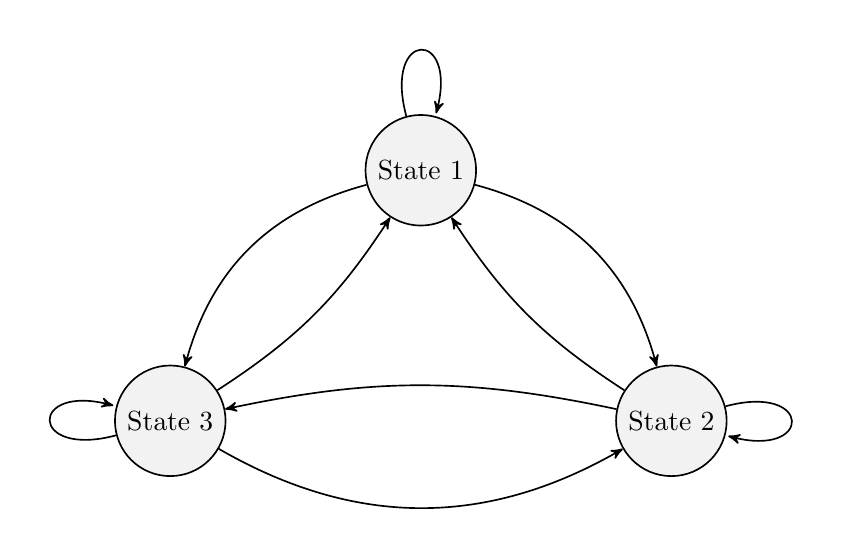
\begin{tikzpicture}
\node[state] (s1) {State 1};
\node[state, below right of=s1] (s2) {State 2};
\node[state, below left of=s1] (s3) {State 3};

\draw (s1) edge[loop above]  (s1);
\draw (s1) edge[bend left]  (s2);
\draw (s1) edge[bend right]  (s3);

\draw (s2) edge[bend left=12]  (s1);
\draw (s2) edge[loop right]  (s2);
\draw (s2) edge[bend right=12]  (s3);

\draw (s3) edge[bend right=12]  (s1);
\draw (s3) edge[bend right]  (s2);
\draw (s3) edge[loop left]  (s3);

\end{tikzpicture}
\caption{Example of a Markov chain depicted as a directed graph.}
\end{figure}
Statisticians with strong mathematical instincts\footnote{i.e. competent ones.} might now be curious about the distribution described by such a Markov chain specified by its transition matrix. This, of course, depends on what initial distribution of states is chosen, a starting point for the chain so to speak. This initial distribution $\pi_0$ (a row vector of $N$ probabilites such that $\pi_i \geq 0 \text{ and }\sum_i \pi_i = 1$) then fully defines all further distributions, through the \textit{evolution equations}. With $\pi_t$ denoting the marginal distribution of $Z_t$, with $\pi_t (i) = P(Z_t = i)$, the mentioned equation holds
\[
\pi_t = \pi_0 \textbf{P}^t
\].
With $\textbf{P}^t$ offering the transition probabilites like so
\[
(\textbf{P}^t)_{ij} = P(Z_t = j \mid Z_0 = i)
\].
A central concept in the application of Markov chains is the \textit{stationary distribution}. A row vector $\pi$ of familiar form is called stationary distribution of the relevant Markov chain if
\[
\pi = \pi \textbf{P}
\]
, honoring its name in an obvious manner. The term \textit{invariant measure} is often used synonymously. This condition can be rewritten as 
\[
\forall j \in \{1, 2, \dots , N\}: \quad \pi_j = \sum_i \pi_i p_{ij} 
\]
In large parts of the literature these conditions are known as the \textit{global balance equations}. The most tempting remaining questions now involve the existence and uniqueness of such a stationary distribution for a given Markov chain. In order to answer these, the following text will define several important properties a Markov chain might fulfill and how some of these relate to their stationary distributions. At first we will consider only chains with finite state spaces.\\
\begin{itemize}
\item{A state $i$ is called \textit{recurrent}, if $P(T_i < \infty \mid Z_0 = i)=1$, with $T_i = \inf (t \geq 1: Z_t = i)$ denoting the first time state $i$ is realised. $\inf$ being the \textit{infimum}, i.e. the greatest lower bound. This simply describes the process almost surely returning to state $i$ after initially starting there. If a state is not recurrent, it is \textit{transient}. Transcience therefore describes the case of positive probability for the event of never returning to a given state.}

\item{A state $i$ is said to have period $k$ if the return to this state can only occur in multiples of $k$ time steps, which can be written as
\[k = gcd\{n >0 : P(Z_n  = i \mid Z_o = i) > 0\}\], as long as this set is not empty. $gcd$ denoting the \textit{greatest common divisor}. In the case of $k=1$ the state is called aperiodic.}

\item{A state $j$ is called \textit{accessible} from state $i$, tentatively written as $i \to j$ if $\exists t \geq 0:$ $\textbf{P}^t_{ij} > 0 $. States $i$ and $j$ are furthermore said to \textit{communicate} if $i \to j$ and $j \to i$ hold. And building on these properties a Markov chain is called \textit{irreducible} if all of its states communicate.}
\item{A state is called \textit{ergodic} if it is recurrent and aperiodic, and the whole chain is called ergodic if all of its states are.}
\end{itemize}
When considering an irreducible finite Markov chain, all its states are recurrent and ergodicity as well as periodicity are global properties, in the sense that they are shared among all states. Wielding this new knowledge delivers the useful insight that for any ergodic, finite Markov chain one may construct its unique stationary distribution like so:
\[
\lim_{t \to \infty} P(Z_t = j \mid Z_0 = i) = \lim_{t \to \infty} \textbf{P}^{t}_{ij} =: \pi^{\infty}_j
\]
Only minimal changes to this conclusion arise in the case of a countably infinite state space. The property of recurrence is then extended in a natural manner:
\begin{itemize}
\item{A recurrent state $i$ is called \textit{positive recurrent}, if the time to return to the state possesses a finite mean, i.e. $\E (T_i \mid Z_o = i) < \infty$. Otherwise it is considered \textit{null recurrent}.}
\end{itemize}
Ergodicity of a state is then in turn defined as reliant on the positive reccurrence of this state, and aperiodicity as before. In an irreducible Markov chain the properties of positive and null recurrence and periodicity as well as ergodicity are now global. Lastly we can conclude that  in this case an irreducible chain possesses a stationary distribution if and only if all of its states are positive recurrent. This distribution is indeed also unique.

\newpage
\appendix
\section{Filtrations}
A family $(\mathscr{I}_t)_{t \in T}$ of $\sigma$-algebras in $\Omega$ is called \textit{filtration} in $\sigma$-algebra $\mathscr{A}$ if
\[\forall t \in T: \quad \mathscr{I}_t \subset \mathscr{A}\] and
\[\forall t_1, t_2 \in T \text{ with } t_1 \leq t_2 : \mathscr{I}_{t_1}\subset \mathscr{I}_{t_2}\].
The quadruple $(\Omega , \mathscr{A}, P, (\mathscr{I}_t)_{t \in T})$ is called filtered probability space.

\end{document}